\subsection{Architectural Design Principles and Initial Implementation}

\subsubsection{Microservices Architecture Rationale}

The system adopted an n-layered microservices architecture following domain-driven design principles. This approach provided clear separation of concerns and enabled independent scaling of translation components.

\subsubsection{Architecture Components:}
\begin{itemize}
    \item \textbf{Controller Layer:} REST endpoint exposure and request validation
    \item \textbf{Service Layer:} Business logic processing and orchestration
    \item \textbf{External API Integration:} Translation engine communication and data transformation
\end{itemize}

\subsubsection{Design Benefits:}
\begin{itemize}
    \item Service independence enabling targeted scaling
    \item Clear API contracts between components
    \item Technology diversity support within service boundaries
    \item Fault isolation preventing cascading failures
\end{itemize}

\subsection{Initial Implementation Challenges}

\subsubsection{Primary Challenge: Data Structure Transformation}

The most significant technical challenge involved converting JSON cultural tips data into string arrays compatible with LibreTranslate's API, then reconstructing the translated content while preserving semantic relationships and data integrity.

\subsubsection{Solution Architecture:}
\begin{lstlisting}[language=Java]
Map<String, List<SentenceContext>> jsonContext = new HashMap<>();
\end{lstlisting}

Each JSON object was mapped to a \texttt{SentenceContext} object containing:
\begin{itemize}
    \item Original text content
    \item Translated text content
    \item Batch array index position
    \item Batch index position
\end{itemize}

\textbf{Reconstruction Logic:} The mapping enabled accurate JSON reconstruction by iterating through context lists and retrieving translated content based on stored indices, ensuring no data loss during the translation pipeline.

\begin{figure}[H]
    \centering
    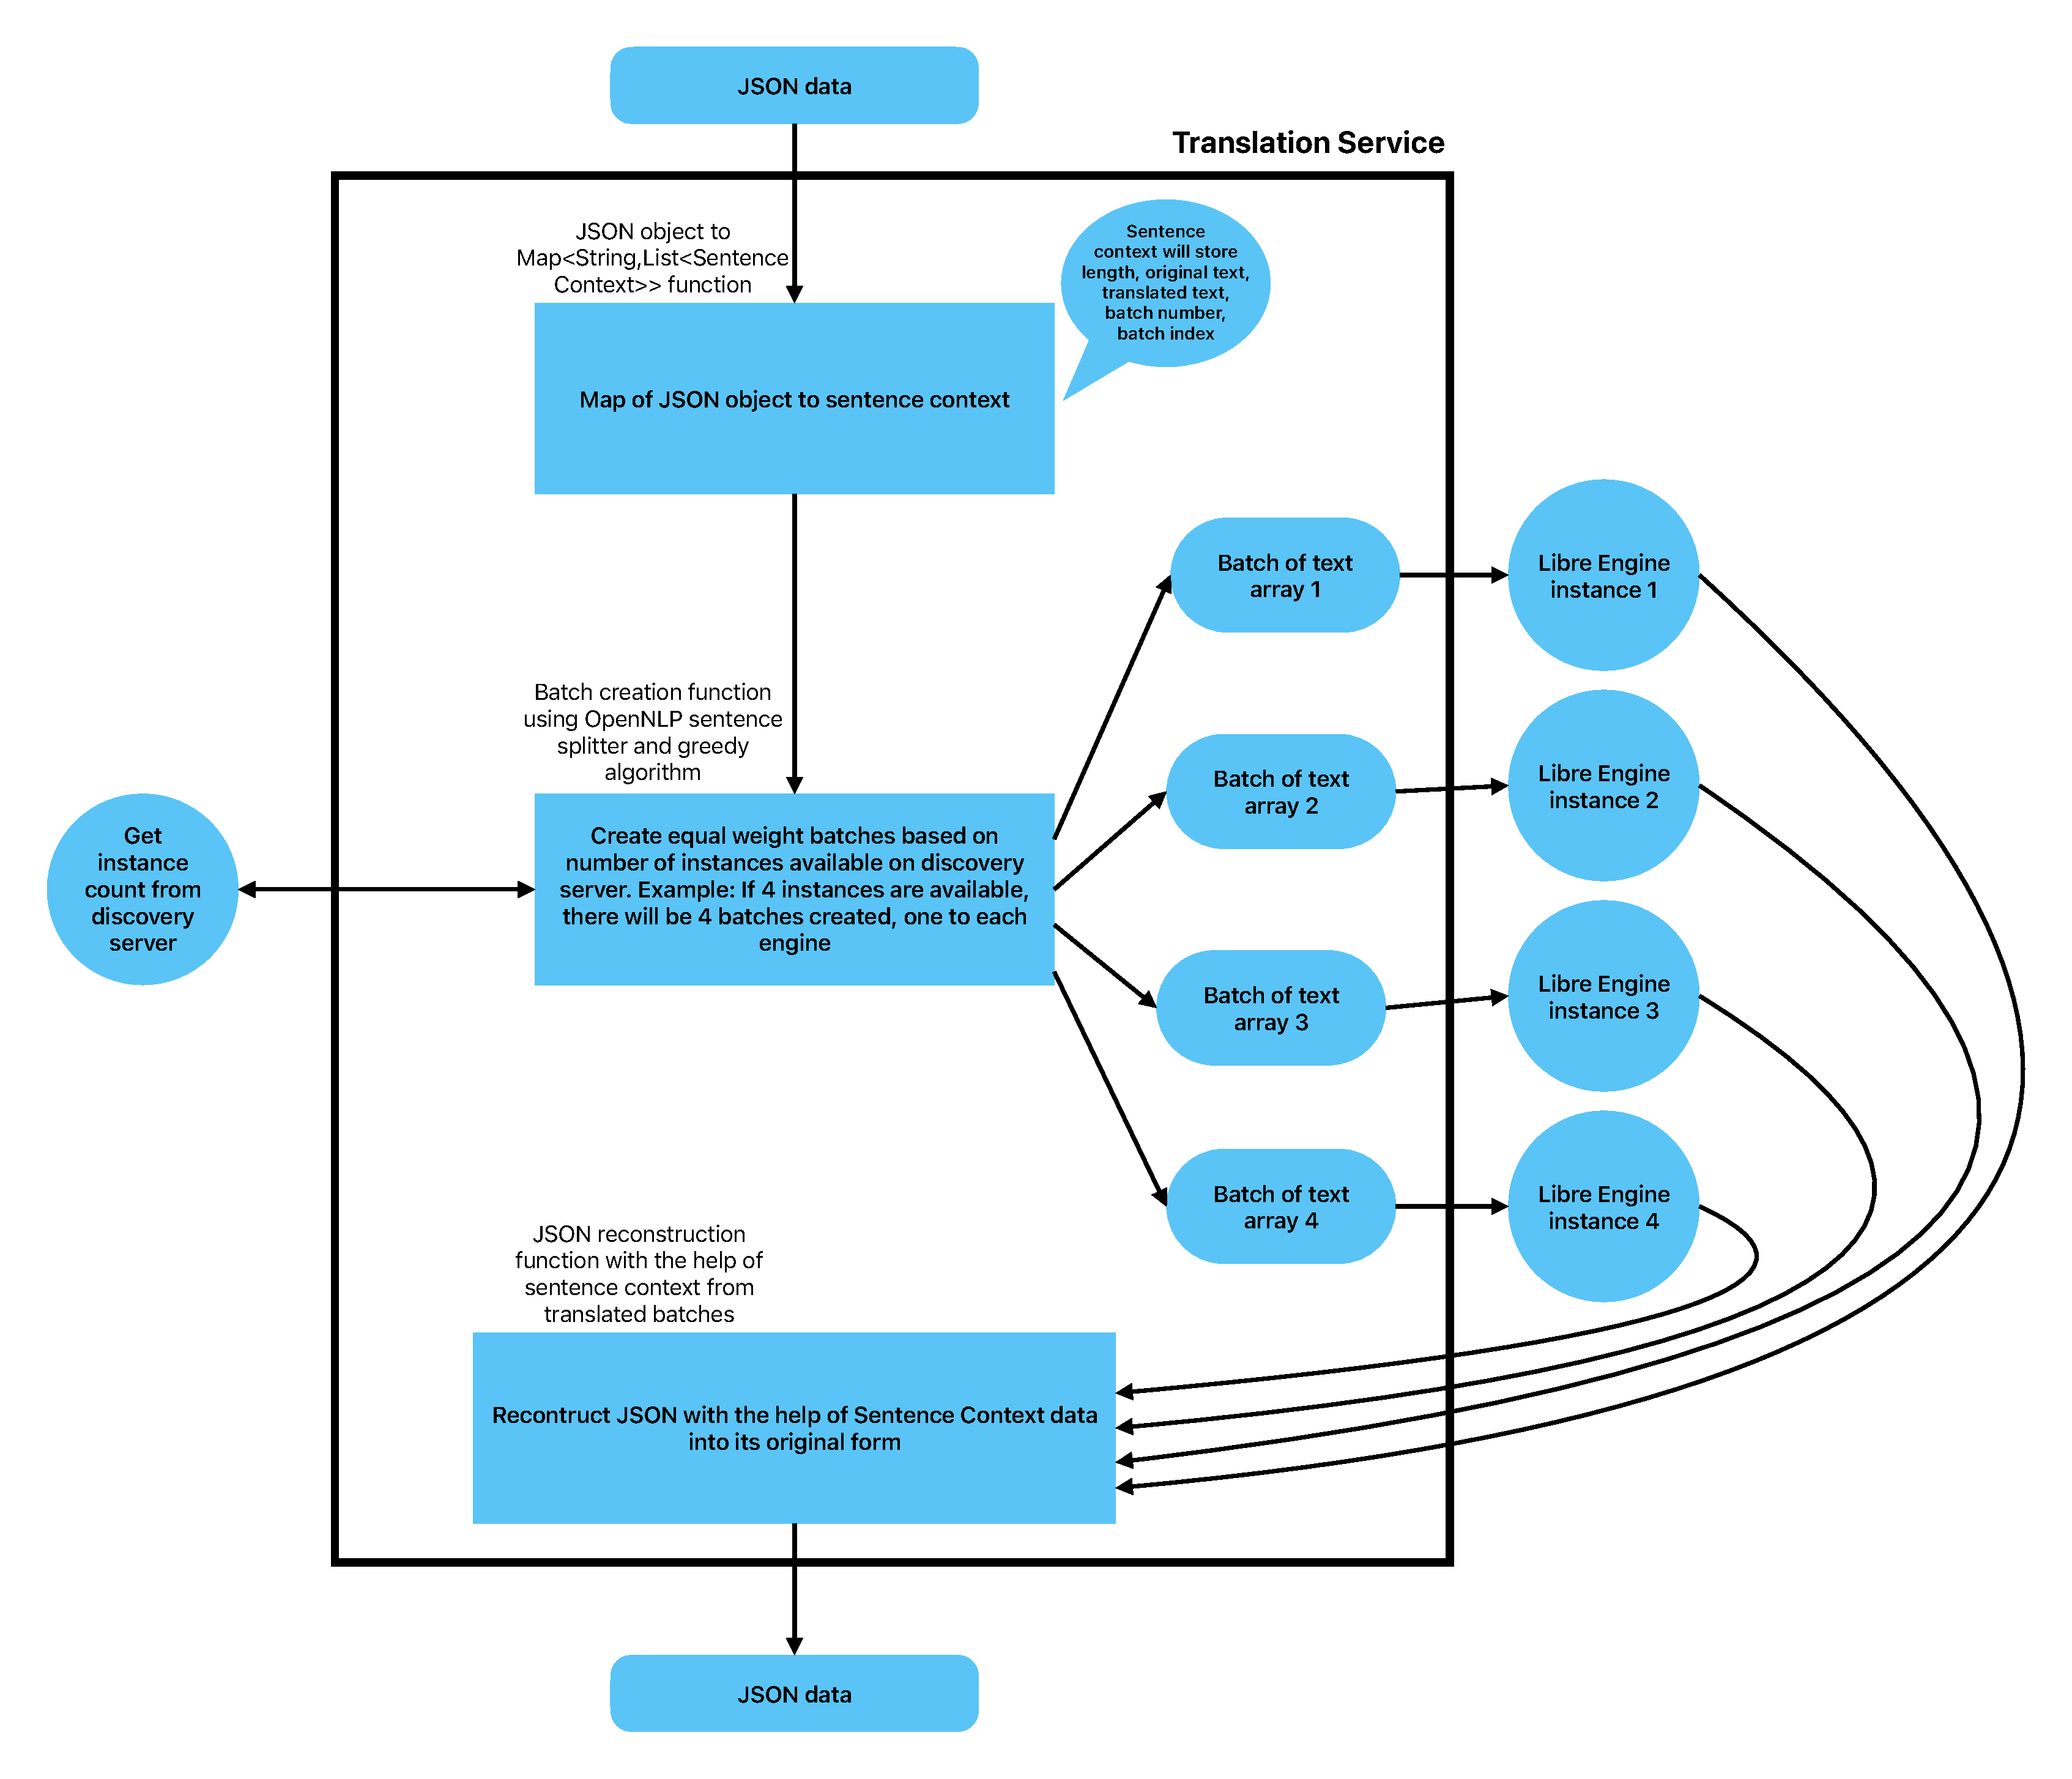
\includegraphics[width=1\linewidth]{chapter/05_implementation/backend/B_architectural_design/Translation_Service.pdf}
    \caption{Translation request lifecycle}
    \label{fig:translation_engine_radar}
\end{figure}